\documentclass[tikz,border=5pt]{standalone}
\usepackage{amsmath,amssymb}
\usepackage{tikz}
\usetikzlibrary{calc,arrows.meta}
\begin{document}
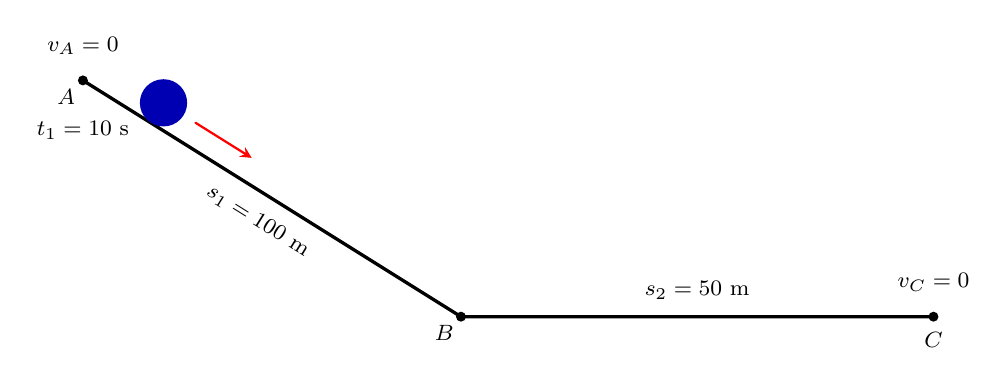
\begin{tikzpicture}[>=stealth, line join=round, line cap=round, font=\footnotesize, scale=1.2]
	% Định nghĩa các điểm tọa độ chính
	\path (0,2.5) coordinate (A)
	(4,0) coordinate (B)
	(9,0) coordinate (C);
	% Vẽ đường đi (nét chính, dày)
	\draw[line width=1.2pt] (A) -- (B) -- (C);
	% Xác định vị trí vật (hình tròn) trên đoạn AB bằng tọa độ cực
	\path (A) -- (B) coordinate[pos=0.18] (X);
	% Góc dốc xấp xỉ 32 độ, hướng vuông góc lên trên là 58 độ
	\coordinate (ball_center) at ([shift={(58:0.25)}]X);
	% Vẽ vật (hình tròn)
	\fill[blue!70!black] (ball_center) circle (0.25cm);
	% Vẽ mũi tên chuyển động song song với mặt dốc
	\coordinate (arrow_start) at ([shift={(-32:0.4)}]ball_center);
	\draw[->, >=stealth, thick, red] (arrow_start) -- ++(-32:0.7);
	% Nhãn thông số trên các đoạn đường
	\path (A) -- (B) node[below, midway, sloped, yshift=-1mm] {$s_1=100\text{ m}$};
	\path (B) -- (C) node[above, midway, yshift=1mm] {$s_2=50\text{ m}$};
	% Nhãn thông số tại các điểm đầu và cuối
	\node[above=2mm] at (A) {$v_A=0$};
	\node[below=4mm] at (A) {$t_1=10\text{ s}$};
	\node[above=2mm] at (C) {$v_C=0$};
	% Nhãn điểm và dấu chấm tròn
	\foreach \p/\g in {A/-135, B/-135, C/-90}
	\fill[black] (\p) circle (1.5pt) ++(\g:0.25) node {$\p$};
\end{tikzpicture}
\end{document}
